\chapter{Unsupervised pre-learning method}

In this chapter, in the context of the DNN learning problem, we derive the classical learning rules for the restricted Boltzmann Machine, which is used at the stage of unsupervised pretraining of the DNN.

An alternative approach to training a restricted Boltzmann machine (\cite{1-A, 4-A, 5-A}) is proposed, based on minimizing errors in image reconstruction on its visible and hidden layers using Gibbs sampling iterations. MSE (mean squared error) and CE (cross-entropy loss) are used as minimization criteria.

For the proposed approach, the derivation of RBM learning rules is considered. It is shown that the obtained rules generalize the classical learning rules obtained in the works of J. Hinton.

An approach is proposed to reduce the dimension of neural network models by reducing the number of adjustable parameters and the number of used neurons after performing the pretraining procedure using RBM networks.

For the main cases, CRBM learning rules are given that can be used to pretrain deep convolutional neural networks. It is also shown that the convolutional layer can be represented as a fully connected layer.

\section{RBM training}

In Chapter 1, it was described that one of the methods for training the DNN is the pre-training method, based on the use of limited Boltzmann machines.

Also, it was previously mentioned that the main task of training a limited Boltzmann machine is to reproduce the distribution of input data based on the states of neurons in the hidden layer as accurately as possible. This is equivalent to maximizing the likelihood function by modifying the synaptic connections of the neural network. Let us show the main steps in deriving learning rules for RBM.

The probability of finding a visible and hidden neuron in the $(x, y)$ state is determined based on the Gibbs distribution \cite{gibbs1902}:

\begin{equation*}
P(x, y)=\frac{e^{-E(x,y)}}{Z}
\end{equation*}
where $E(x,y)$ is the energy of the system in the state $(x,y)$, $Z$ is a parameter that determines the probability normalization condition, that is, the condition under which the sum of the probabilities $P(x, y)$ is equal to one. This parameter is defined as follows:

\begin{equation*}
Z=\sum_{x,y}e^{-E(x,y)}
\end{equation*}

The probability of finding visible neurons in a certain state is equal to the sum of the probabilities of configurations $P(x,y)$ over the states of hidden neurons:

\begin{equation*}
P(x)=\sum_y P(x,y)=\sum_y \frac{e^{-E(x,y)}}{Z}=\frac{\sum_y e^{-E(x,y))){\sum_{x,y} e^{-E(x,y))))
\end{equation*}

To find the rules for modifying model parameters, it is necessary to maximize the probability of reproducing the states of visible neurons $P(x)$ by a limited Boltzmann machine. In order to determine the maximum of the likelihood function of the data distribution $P(x)$, we will use the gradient lifting method in the space of weight coefficients and threshold values of the network, where we use the log-likelihood function as the objective function:

\begin{equation*}
\ln P(x)=\ln \sum_y e^{-E(x,y)}-\ln \sum_{x,y} e^{-E(x,y)}
\end{equation*}

Then the gradient is

\begin{equation*}
\frac{\partial \ln P(x)}{\partial w_{ij))=\frac{\partial}{\partial w_{ij))\ln \sum_y e^{-E(x,y)}-\frac{\partial}{\partial w_{ij))\ln\sum_{x,y} e^{-E(x,y)}
\end{equation*}

Transforming the last expression, we get

\begin{equation*}
\frac{\partial \ln P(x)}{\partial w_{ij}}=-\frac{1}{\sum_y e^{-E(x,y)}}\sum_y e^{-E(x,y)}\frac{\partial E(x,y)}{\partial w_{ij}}+\frac{1}{\sum_{x,y} e^{-E(x,y)))\sum_{x,y} e^{-E(x ,y)}\frac{\partial E(x,y)}{\partial w_{ij))
\end{equation*}

Because

\begin{equation*}
P(x,y)=P(y\lvert x)P(x)
\end{equation*}

That

\begin{equation*}
P(y \lvert x) = \frac{P(x,y)}{P(x)}=\frac{\slantfrac{1}{Z}e^{-E(x,y)}}{\slantfrac{1}{Z}\sum_y e^{-E(x,y)}}=\frac{e^{-E(x,y))){\sum_y e^{-E(x,y))))
\end{equation*}

As a result, you can get the following expression:

\begin{equation}
\label{derivative_log}
\frac{\partial \ln P(x)}{\partial w_{ij))=-\sum_y P(y \lvert x)\frac{\partial E(x,y)}{\partial w_{ij)) + \sum_{x,y} P(x,y)\frac{\partial E(x,y)}{\partial w_{ij))
\end{equation}

In this expression, the first term determines the positive phase of the Boltzmann machine, when the network operates on the basis of images from the training set. The second term characterizes the negative phase of operation, when the network operates in a free mode, regardless of the environment.

If we consider the energy function of the RBM network, then in this case, the learning task is to find, based on the input data, the configuration of neurons in the hidden layer with minimum energy. As a result, on the training set, the network will have less energy compared to other states. The energy function of the binary state $(x,y)$ is defined similarly to the energy function of the Hopfield network:

\begin{equation}
E(x,y)=-\sum_i x_iT_i-\sum_j y_jT_j-\sum_{i,j} x_iy_jw_{ij}
\end{equation}

In this case

\begin{equation*}
\frac{\partial E(x,y)}{\partial w_{ij}}=-x_iy_j
\end{equation*}

Substituting the resulting value into the \ref{derivative_log} formula, we get

\begin{equation*}
\frac{\partial \ln P(x)}{\partial w_{ij}}=\sum_y P(y \lvert x)x_i y_j-\sum_{x,y} P(x,y)x_iy_j
\end{equation*}

Since the mathematical expectation of the input data is equal to:

\begin{equation}
\label{mean}
E(x)=\sum_i x_iP_i
\end{equation}

That

\begin{equation}
     \label{grad_weights}
\frac{\partial \ln P(x)}{\partial w_{ij}}=E\left[x_iy_j\right]_{\text{data}}-E\left[x_iy_j\right]_{\text{model}}
\end{equation}

Arguing in a similar way, we find

\begin{equation*}
\frac{\partial \ln P(x)}{\partial T_{i))=-\sum_y P(y \lvert x)\frac{\partial E(x,y)}{\partial T_{i)) + \sum_{x,y} P(x,y)\frac{\partial E(x,y)}{\partial T_{i))
\end{equation*}

And

\begin{equation*}
\frac{\partial \ln P(x)}{\partial T_{j))=-\sum_y P(y \lvert x)\frac{\partial E(x,y)}{\partial T_{j)) + \sum_{x,y} P(x,y)\frac{\partial E(x,y)}{\partial T_{j))
\end{equation*}

Because

\begin{equation*}
\frac{\partial E(x,y)}{\partial T_{i}}=-x_i
\end{equation*}

And

\begin{equation*}
\frac{\partial E(x,y)}{\partial T_{j}}=-y_j
\end{equation*}

then, given the formula \ref{mean}, we get the gradients for the threshold values:

\begin{equation}
\label{grad_biases}
\begin{aligned}
\frac{\partial \ln P(x)}{\partial T_i}=E\left[x_i\right]_{\text{data}}-E\left[x_i\right]_{\text{model}}\\
\frac{\partial \ln P(x)}{\partial T_j}=E\left[y_j\right]_{\text{data}}-E\left[y_j\right]_{\text{model}}
\end{aligned}
\end{equation}

As follows from the last expressions, the first term characterizes the network operation based on the data from the training sample, and the second term characterizes the network operation based on the model data (data generated by the network), that is, in a free mode, regardless of the environment.
Since the calculation of the mathematical expectation in the formulas \ref{grad_weights} and \ref{grad_biases} is a difficult task, Hinton suggested using an approximation of these terms obtained by applying a procedure he called Contrastive Divergence (CD)) \cite{n1}.

This approximation is based on the Gibbs sampling. In this case, the first terms in the expressions \ref{grad_weights} and \ref{grad_biases} characterize the data distribution at time $t=0$, and the second terms characterize the reconstructed or model-generated data at time $t=k$. Based on this, the CD-$k$ procedure can be represented as follows:

\begin{equation}
x(0) \rightarrow y(0) \rightarrow x(1) \rightarrow y(1) \rightarrow \ldots \rightarrow x(k) \rightarrow y(k)
\end{equation}

As a result, we can formulate the following rules for training the RBM network. In the case of CD-1 (case $k=1$) and considering that according to the gradient lifting method

\begin{equation*}
w_{ij}(t+1)=w_{ij}(t)+\alpha\frac{\partial \ln P(x)}{\partial w_{ij}(t)}
\end{equation*}

You can get that
\begin{equation*}
w_{ij}(t+1)=w_{ij}(t)+\alpha(x_i(0)y_j(0)-x_i(1)y_j(1))
\end{equation*}
\begin{equation*}
T_i(t+1)=T_i(t)+\alpha(x_i(0)-x_i(1))
\end{equation*}
\begin{equation*}
T_j(t+1)=T_j(t)+\alpha(y_j(0)-y_j(1)).
\end{equation*}

Similarly, for the CD-$k$ algorithm
\begin{equation*}
w_{ij}(t+1)=w_{ij}(t)+\alpha(x_i(0)y_j(0)-x_i(k)y_j(k))
\end{equation*}
\begin{equation*}
T_i(t+1)=T_i(t)+\alpha(x_i(0)-x_i(k))
\end{equation*}
\begin{equation*}
T_j(t+1)=T_j(t)+\alpha(y_j(0)-y_j(k)).
\end{equation*}

It can be seen from the last expressions that in the process of training the restricted Boltzmann machine, the difference between the original data and the data generated by the model is minimized.

Similarly, you can get the learning rules for the group case (for example, when using mini-batch optimization, case CD-1):

\begin{equation*}
w_{ij}(t+1)=w_{ij}(t)+\frac{\alpha}{L}\sum_{l=1}^L(x_i^l(0)y_j^l(0)-x_i^l(1)y_j^l(1))
\end{equation*}
\begin{equation*}
T_i(t+1)=T_i(t)+\frac{\alpha}{L}\sum_{l=1}^L(x_i^l(0)-x_i^l(1))
\end{equation*}
\begin{equation*}
T_j(t+1)=T_j(t)+\frac{\alpha}{L}\sum_{l=1}^L(y_j^l(0)-y_j^l(1)).
\end{equation*}
where $L$ is the number of images in the group.

Summarizing the above, we present the complete RBM learning algorithm for the CD-1 case (algorithm~\ref{rbm_learning}).

\begin{algo}[h]
%\SetAlgoLined

\KwIn{\textit{\textbf{x(0)}} -- image vector from the training sample,
$\alpha$ - learning rate
}
\KwRes{weight matrix \textit{\textbf{W}}, visible layer neuron threshold vector $\textit{\textbf{V}}$, hidden layer neuron threshold vector $\textit{\textbf{H}}$}
\ForEach{of the hidden layer neuron $j$}{
Calculate $P(y_{j}(0)=1|x_{i}(0))$ (for binomial neurons sigmoid($\sum_{i}{w_{ij}x_{i}(0)}+H_j$))\;
Generate $y_{j}(0) \in \{0, 1\}$ from $P(y_{j}(0)|x_i(0))$\;
}
\ForEach{neuron of the visible layer $i$}
{
Calculate $P(x_{i}(1)=1|y_j(0))$ (for binomial neurons sigmoid($\sum_{j}{w_{ij}y_{j}(0)} + V_i$))\;
Generate $x_{i}(1) \in \{0, 1\}$ from $P(x_{i}(1)|y_j(0))$\;
}
\ForEach{hidden neurons $j$}
{
Calculate $P(y_{j}(1)=1|x_i(1))$ (for binomial neurons sigmoid($\sum_{i}{w_{ij}x_{i}(1)} + H_j$))\;
}
$\textit{\textbf{W}} \leftarrow \textit{\textbf{W}} + \alpha(\textbf{\textit{x(0)}}\textit{\textbf{y(0)}}^T - \textit{\textbf{x(1)}}P(\textit{\textbf{y(1)))=1|\textit{\textbf{x(1))))^T)$\;
$\textit{\textbf{V}} \leftarrow \textit{\textbf{V}} + \alpha(\textit{\textbf{x(0)}} - \textit{\textbf{x(1))))$\;
$\textit{\textbf{H}} \leftarrow \textit{\textbf{H}} + \alpha(\textit{\textbf{y(0)}} - P(\textit{\textbf{y(1)}}=1|\textit{\textbf{x(1)))))$\;
% \While{not at the end of this document}{
% read current\;
% \eIf{understand}{
% go to next section\;
% current section becomes this one\;
% }{
% go back to the beginning of the current section\;
%}
%}
     \caption{RBM training procedure}
\label{rbm_learning}
\end{algo}

\section{General description of the proposed method}

Compared to the traditional RBM \cite{n1} learning method proposed by Jeffrey Hinton, which is based on the application of the energy function (energy-based method) and actually operates with a linear representation of neural elements, our method allows us to take into account their nonlinear nature.
 
Let's consider a limited Boltzmann machine, which we will represent as three layers of neural elements \cite{n10}: visible, hidden and visible (figure~\ref{fig:pic2_1}). In the above representation, the matrix of weight coefficients $W_{ji}$ for the second layer is obtained by transposing the matrix $W_{ij}$ of the first layer. In fact, when training is performed, its elements are changed once.

\begin{figure}[H]
   \centering
   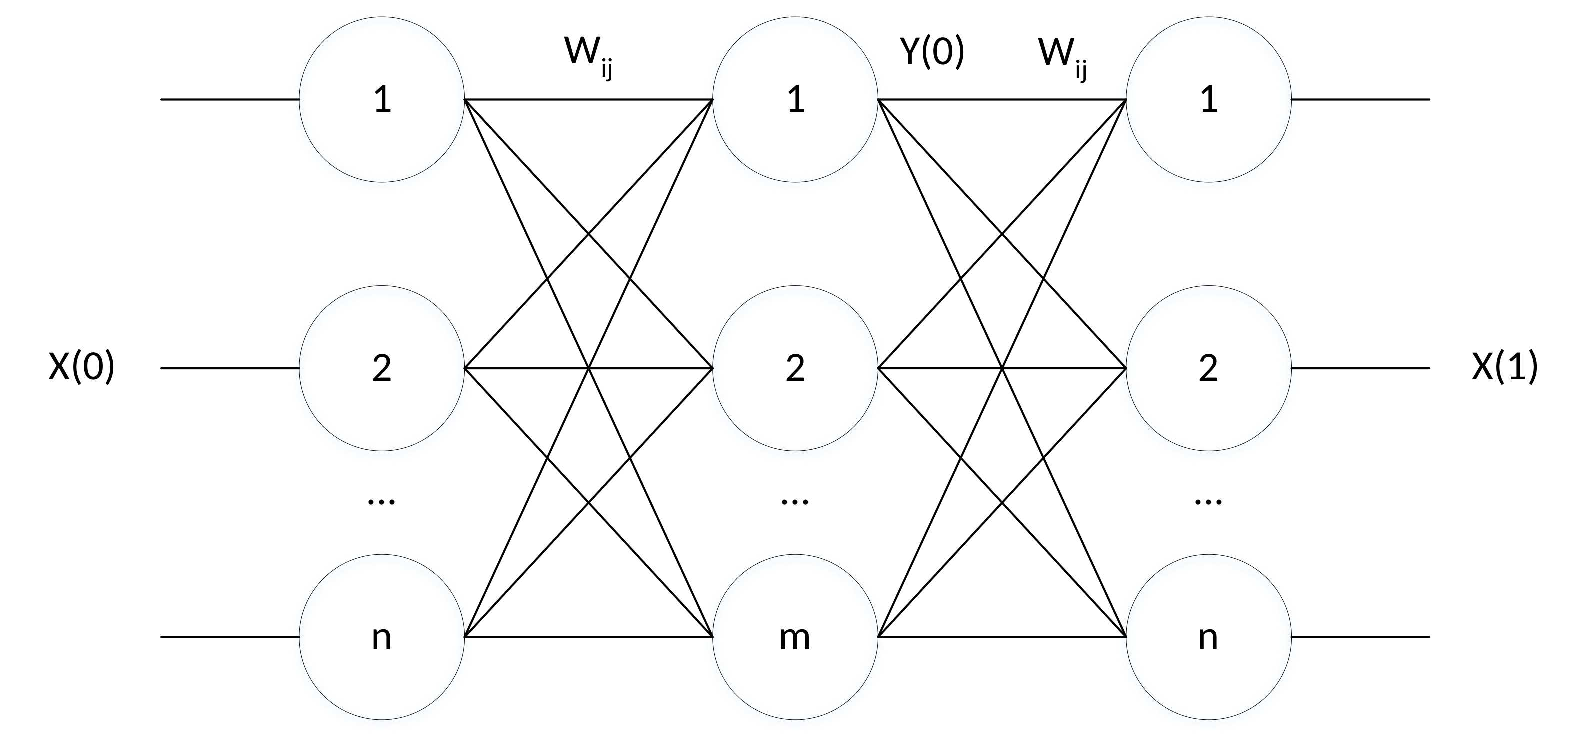
\includegraphics[width=0.9\textwidth]{man-source/images/ch2/pic2-1.pdf}
   \caption{Expanded RBM representation}
   \label{fig:pic2_1}
\end{figure}

Let's imagine Gibbs sampling using the expanded representation of RBM (figure~\ref{fig:pic2_2}).

\begin{figure}[H]
   \centering
   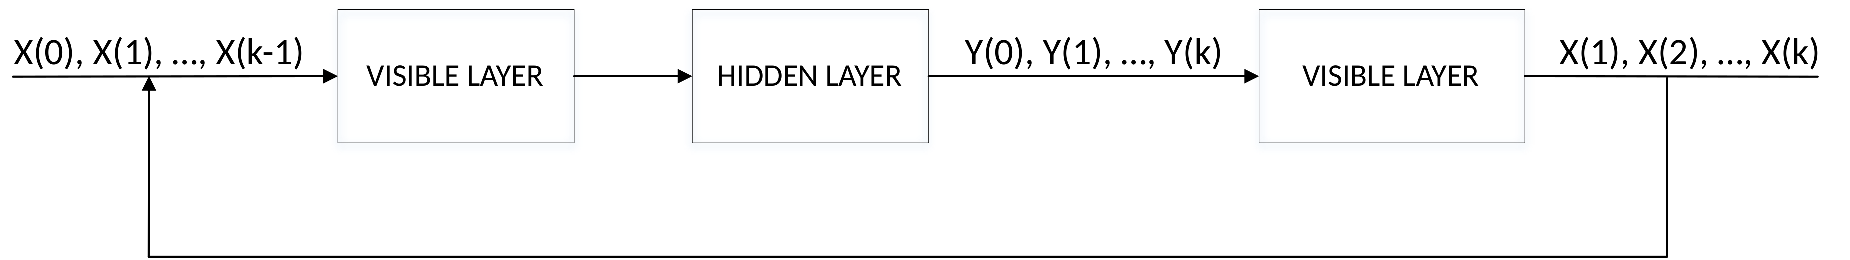
\includegraphics[width=\textwidth]{man-source/images/ch2/pic2-2.pdf}
   \caption{Gibbs sampling}
   \label{fig:pic2_2}
\end{figure}

Sampling Gibbs is the following procedure. Let $x(0)$ be the input vector that arrives at the visible layer at time $t=0$. Then the output values of neurons in the hidden layer will be determined as follows:

\begin{equation}
     y_j(0)=F(S_j(0)),
\end{equation}

\begin{equation}
     S_j(0)=\sum_i w_{ij}x_i(0)+T_j.
\end{equation}

The inverse (last) layer reconstructs the input vector based on the data from the hidden layer and the current value of the adjustable parameters (visible layer thresholds and weight matrix). The result is the restored vector $x(1)$ at time $t=1$:

\begin{equation}
     x_i(1)=F(S_i(1)),
\end{equation}

\begin{equation}
     S_i(1)=\sum_j w_{ij}y_j(0)+T_i.
\end{equation}

Then the vector $x(1)$ is fed to the visible layer, and the output values of neurons in the hidden layer are calculated:

\begin{equation}
     y_j(1)=F(S_j(1)),
\end{equation}

\begin{equation}
     S_j(1)=\sum_i w_{ij}x_i(1)+T_j.
\end{equation}

Continuing this process, we can obtain the following expressions at step k:

\begin{equation*}
     y_j(k)=F(S_j(k)),\ S_j(k)=\sum_i w_{ij}x_i(k)+T_j.
\end{equation*}

\begin{equation*}
     x_i(k)=F(S_i(k)),\ S_i(k)=\sum_j w_{ij}y_j(k-1)+T_i.
\end{equation*}

\section{Derivation of pre-training rules}

Hinton proposed an energy model based on the idea of maximizing the likelihood function of the input data distribution $P(x)$. The derivation of the classical learning rules was given in chapter I. Based on the idea of using a restricted Boltzmann machine as an auxiliary model for pre-training, we proposed the use of two different criteria for its training \cite{4-A}. The first criterion is based on minimizing the mean square error (MSE), and the second one is based on minimizing the cross-entropy error function.

Let us show that the application of different minimization criteria allows, nevertheless, to obtain the same learning rules.

\subsection{MSE criterion}

In the case of using MSE as a learning criterion, the main goal of learning a limited Boltzmann machine is to minimize the total mean square error of data reconstruction on the hidden and visible (restoring) layers, which in the case of CD-k is defined as follows:

\begin{equation*}
     E_s(k)=\frac{1}{2L}\Bigg(\sum_{l=1}^L\sum_{j=1}^m\sum_{p=1}^k (y_j^l(p)-y_j^l(p-1))^2+\sum_{l=1}^L\sum_{i=1}^n\sum_{p=1}^k (x_i^l(p)-x_i^l(p -1))^2\Bigg)
\end{equation*}
where \textit{k} defines the parameter of the Gibbs sampling procedure, \textit{n} is the number of neurons in the visible layer, \textit{m} is the number of neurons in the hidden layer, \textit{L} is the dimension of the training sample.

In the case of CD-1, the total mean square error

\begin{equation}
     E_s(1)=\frac{1}{2L}\Bigg(\sum_{l=1}^L\sum_{j=1}^m (y_j^l(1)-y_j^l(0))^2+\sum_{l=1}^L\sum_{i=1}^n (x_i^l(1)-x_i^l(0))^2\Bigg)
\end{equation}

As follows from the above expressions, the error consists of two parts: errors in restoring information on the visible and hidden layers, i.e. can be presented in the following form:
\begin{equation}
\label{mse_rbm_criteria}
E_s(k) = E_h(k) + E_v(k)
\end{equation}
Where

\begin{equation}
E_h(k) = \frac{1}{2L}\sum_{l=1}^L\sum_{j=1}^m\sum_{p=1}^k (y_j^l(p)-y_j^l(p-1))^2
\end{equation}

\begin{equation}
E_v(k) = \frac{1}{2L}\sum_{l=1}^L\sum_{i=1}^n\sum_{p=1}^k (x_i^l(p)-x_i^l(p-1))^2
\end{equation}

Let's find the learning rules corresponding to the criterion \ref{mse_rbm_criteria} and prove their equivalence to the classical RBM learning rules under certain special conditions.

\textbf{Theorem 1}. Maximizing the likelihood function of data distribution $P(x)$ in the space of synaptic connections of a bounded Boltzmann machine is equivalent to minimizing the total squared error of the network in the same space using linear neurons.

\textbf{Proof}: Consider sequential RBM learning, where modification of synaptic connections occurs after each input pattern is fed to the network (online learning). According to the gradient descent method, to minimize the network's total squared error, synaptic connections should change as follows:

\begin{equation}
w_{ij}(t+1)=w_{ij}(t)-\alpha\frac{\partial E}{\partial w_{ij}(t)},
\end{equation}

\begin{equation}
T_{i}(t+1)=T_{i}(t)-\alpha\frac{\partial E}{\partial T_{i}(t)},
\end{equation}

\begin{equation}
T_{j}(t+1)=T_{j}(t)-\alpha\frac{\partial E}{\partial T_{j}(t)},
\end{equation}

In the case of CD-k, the quadratic error $E$ for one image is:

\begin{equation*}
E=\frac{1}{2}\sum_{j=1}^m\sum_{p=1}^k (y_j(p)-y_j(p-1))^2+\frac{1}{2}\sum_{i=1}^n\sum_{p=1}^k (x_i(p)-x_i(p-1))^2
\end{equation*}

Then
\begin{multiline*}
     \frac{\partial E}{\partial w_{ij))=\frac{\partial E}{\partial y_j(p)}\frac{\partial y_j(p)}{\partial S_j(p)}\frac{\partial S_j(p)}{\partial w_{ij))+\frac{\partial E}{\partial x_i(p)}\frac{\partial x_i(p)}{\partial S_i(p) }\frac{\partial S_i(p)}{\partial w_{ij}}=\\=\sum_{p=1}^k (y_j(p)-y_j(p-1))x_i(p)F'(S_j(p))+\\+\sum_{p=1}^k (x_i(p)-x_i(p-1))y_j(p-1)F'(S_i(p))
\end{multline*}

If the restricted Boltzmann machine uses linear neurons with a linear activation function, then

\begin{equation*}
     \frac{\partial S_i(p)}{\partial w_{ij}}=F'(S_i(p))=\frac{\partial S_j(p)}{\partial w_{ij}}=F'(S_j(p))=1,
\end{equation*}

Then

\begin{equation*}
     \frac{\partial E}{\partial w_{ij}}=\sum_{p=1}^k (y_j(p)x_i(p)-y_j(p-1)x_i(p-1))=y_j(k)x_i(k)-y_j(0)x_i(0),
\end{equation*}

The result is a CD-k RBM learning rule:

\begin{equation*}
     w_{ij}(t+1)=w_{ij}(t)+\alpha(x_i(0)y_j(0)-x_i(k)y_j(k)),
\end{equation*}

Similarly for thresholds:

\begin{equation*}
\begin{aligned}
     T_{j}(t+1)=T_{j}(t)+\alpha(y_j(0)-y_j(k)),\\
     T_{i}(t+1)=T_{i}(t)+\alpha(x_i(0)-x_i(k))
\end{aligned}
\end{equation*}

As you can see, the last expressions coincide with the classical learning rule for a limited Boltzmann machine for CD-k. It follows that for a linear RBM, maximizing the likelihood function of the data distribution $P(x)$ is equivalent to minimizing the total squared error of the network. The theorem has been proven.

\textbf{Corollary 1.1}. The linear restricted Boltzmann machine is equivalent in terms of learning to an autoassociative neural network when used in Gibbs sampling in learning.

\textbf{Corollary 1.2}. For a nonlinear restricted Boltzmann machine, the rule for modifying synaptic connections in the case of CD-k will be as follows:
\begin{multiline*}
     w_{ij}(t+1)=w_{ij}(t)-\\-\alpha\Bigg(\sum_{p=1}^k (y_j(p)-y_j(p-1))x_i(p)F'(S_j(p))+(x_i(p)-x_i(p-1))y_j(p-1)F'(S_i(p))\Bigg)
\end{multline*}

\begin{equation*}
\begin{aligned}
     T_i(t+1)=T_i(t)-\alpha\left(\sum_{p=1}^k (x_i(p)-x_i(p-1))F'(S_i(p))\right),\\
     T_j(t+1)=T_j(t)-\alpha\left(\sum_{p=1}^k (y_j(p)-y_j(p-1))F'(S_j(p))\right),
\end{aligned}
\end{equation*}

\textbf{Corollary 1.3}. For a nonlinear restricted Boltzmann machine, the rule for modifying synaptic connections in the case of CD-1 will be as follows:
\begin{equation*}
     w_{ij}(t+1)=w_{ij}(t)-\alpha((y_j(1)-y_j(0))F'(S_j(1))x_i(1)+(x_i(1)-x_i(0))F'(S_i(1))y_j(0)),
\end{equation*}

\begin{equation*}
     T_i(t+1)=T_i(t)-\alpha(x_i(1)-x_i(0))F'(S_i(1)),
\end{equation*}

\begin{equation*}
     T_j(t+1)=T_j(t)-\alpha(y_j(1)-y_j(0))F'(S_j(1)).
\end{equation*}

When using batch learning, the gradient descent method will take the following form:

\begin{equation}
     w_{ij}(t+1)=w_{ij}(t)-\frac{\alpha}{L}\frac{\partial E_s}{\partial w_{ij}(t)}
\end{equation}

\begin{equation}
     T_{i}(t+1)=T_{i}(t)-\frac{\alpha}{L}\frac{\partial E_s}{\partial T_{i}(t)}
\end{equation}

\begin{equation}
     T_{j}(t+1)=T_{j}(t)-\frac{\alpha}{L}\frac{\partial E_s}{\partial T_{j}(t)}
\end{equation}
where \textit{L} defines mini batch size.

\textbf{Theorem 2}. When using CD-k for a nonlinear restricted Boltzmann machine in the case of group learning, the rule for modifying synaptic connections is determined based on the following expressions:
\begin{multiline*}
     w_{ij}(t+1)=w_{ij}(t)-\\-\frac{\alpha}{L}\Bigg(\sum_{l=1}^L\sum_{p=1}^k (y_j^l(p)-y_j^l(p-1))x_i^l(p)F'(S_j^l(p))+(x_i^l(p)-x_i^l(p-1))y_j^ l(p-1)F'(S_i^l(p))\Bigg),
\end{multline*}

\begin{equation*}
     T_{i}(t+1)=T_{i}(t)-\frac{\alpha}{L}\left(\sum_{l=1}^L\sum_{p=1}^k (x_i^l(p)-x_i^l(p-1))F'(S_i^l(p))\right),
\end{equation*}

\begin{equation*}
     T_{j}(t+1)=T_{j}(t)-\frac{\alpha}{L}\left(\sum_{l=1}^L\sum_{p=1}^k (y_j^l(p)-y_j^l(p-1))F'(S_j^l(p))\right)
\end{equation*}

The process of proving this theorem is similar to the proof of Theorem 1.

\textbf{Corollary 2.1}. When using CD-1 for a nonlinear restricted Boltzmann machine in the case of group learning, the rule for modifying synaptic connections is determined based on the following expressions:

\begin{multiline*}
     w_{ij}(t+1)=w_{ij}(t)-\\-\frac{\alpha}{L}\left(\sum_{l=1}^L (y_j^l(1)-y_j^l(0))x_i^l(1)F'(S_j^l(1))+(x_i^l(1)-x_i^l(0))y_j^l(0)F'(S_i^l(1)) \Bigg)\right.,
\end{multline*}

\begin{equation*}
     T_i(t+1)=T_i(t)-\frac{\alpha}{L}\left(\sum_{l=1}^L (x_i^l(1)-x_i^l(0))F'(S_i^l(1))\right),
\end{equation*}

\begin{equation*}
     T_j(t+1)=T_j(t)-\frac{\alpha}{L}\left(\sum_{l=1}^L (y_j^l(1)-y_j^l(0))F'(S_j^l(1))\right)
\end{equation*}

\textbf{Corollary 2.2}. When using CD-k for a linear restricted Boltzmann machine in the case of group learning, the rule for modifying synaptic connections is determined based on the following expressions:

\begin{equation*}
     w_{ij}(t+1)=w_{ij}(t)+\frac{\alpha}{L}\sum_{l=1}^L (x_i^l(0)y_j^l(0)-x_i^l(k)y_j^l(k)),
\end{equation*}

\begin{equation*}
     T_{i}(t+1)=T_{i}(t)+\frac{\alpha}{L}\sum_{l=1}^L (x_i^l(0)-x_i^l(k)),
\end{equation*}

\begin{equation*}
     T_{j}(t+1)=T_{j}(t)+\frac{\alpha}{L}\sum_{l=1}^L (y_j^l(0)-y_j^l(k))
\end{equation*}

\textbf{Corollary 2.3}. When using CD-1 for a linear restricted Boltzmann machine in the case of group learning, the rule for modifying synaptic connections is determined based on the following expressions:

\begin{equation*}
     w_{ij}(t+1)=w_{ij}(t)+\frac{\alpha}{L}\sum_{l=1}^L (x_i^l(0)y_j^l(0)-x_i^l(1)y_j^l(1)),
\end{equation*}

\begin{equation*}
     T_{i}(t+1)=T_{i}(t)+\frac{\alpha}{L}\sum_{l=1}^L (x_i^l(0)-x_i^l(1)),
\end{equation*}

\begin{equation*}
     T_{j}(t+1)=T_{j}(t)+\frac{\alpha}{L}\sum_{l=1}^L (y_j^l(0)-y_j^l(1))
\end{equation*}

Thus, the learning rules for the limited Boltzmann machine are obtained, which are based on minimizing the quadratic error of information recovery on the visible and hidden layers. The proposed method makes it possible to take into account the nonlinear nature of neural elements. It is shown that the classical expressions for learning a limited machine are a special case of the proposed method. A theorem on the equivalence of maximizing the likelihood function of the distribution of input data $P(x)$ and minimizing the total quadratic error of the network in the same space of synaptic connections for a linear bounded Boltzmann machine is proved.